\documentclass[english,brazilian]{sbc2025}%

\usepackage[misc,geometry]{ifsym}
\usepackage{aas_macros}
\usepackage[bottom]{footmisc}
\usepackage{tabularray}
\usepackage{afterpage}
\usepackage{url}
\usepackage{pifont}
\usepackage{booktabs}
\usepackage{multirow}
\usepackage{tikz}
\usetikzlibrary{arrows.meta,positioning,fit,backgrounds}

\setcitestyle{square}

\definecolor{engtitle}{rgb}{0.5,0.5,0.5}
\definecolor{orcidlogo}{rgb}{0.37,0.48,0.13}
\definecolor{unilogo}{rgb}{0.16, 0.26, 0.58}
\definecolor{maillogo}{rgb}{0.58, 0.16, 0.26}
\definecolor{darkblue}{rgb}{0.0,0.0,0.0}
\hypersetup{colorlinks,breaklinks,
            linkcolor=darkblue,urlcolor=darkblue,
            anchorcolor=darkblue,citecolor=darkblue}

% ---------------------------------------------------------------------
% Macros de redação -- remover antes da submissão
%   \tbd{...}  : conteúdo que depende dos resultados ainda em geração
%   \chk{...}  : afirmação/parâmetro a ser confirmado pelos coautores
% ---------------------------------------------------------------------
\newcommand{\tbd}[1]{\textcolor{red}{[PENDENTE: #1]}}
\newcommand{\chk}[1]{\textcolor{orange!80!black}{[VERIFICAR: #1]}}
\newcommand{\figplaceholder}[2]{%
  \fbox{\parbox[c][#1][c]{0.95\columnwidth}{\centering\small\textcolor{red}{#2}}}}
\newcommand{\cmark}{\ding{51}}
\newcommand{\xmark}{\ding{55}}

% Notação
\newcommand{\Tb}{T_{\mathrm{b}}}
\newcommand{\Cb}{C_{\mathrm{b}}}
\newcommand{\Cn}{C^{\max}_{\text{nó}}}
\newcommand{\Lt}{L^{95}_{\mathrm{tx}}}
\newcommand{\Th}{\Theta}
\newcommand{\Ut}{U}
\newcommand{\Kn}{K_{\text{nó}}}
\newcommand{\tbdc}{\textcolor{red}{?}} % célula de tabela pendente
\newcommand{\nmax}{n_{\max}}

\jid{iSys}
\jtitle{iSys - Journal of Information Systems, 202X, XX:1}
\issn{1984-2902}
\doi{10.5753/isys.202X.XXXXXX}
\copyrightstatement{Este trabalho está licenciado sob uma Licença Creative Commons Atribuição 4.0 Internacional}
\jyear{202X}

\category{Artigo de Pesquisa}

% Conforme o template iSys, o título deve estar em inglês mesmo em artigos em português;
% a versão em português aparece como subtítulo (\engtitle).
\title[Dimensionamento do Consenso Bizantino em Registros REDD+]{Sizing Byzantine Consensus for Blockchain-Based REDD+ Registries: Governance, Demand, and Feasibility Frontiers}
\engtitle{Dimensionamento do Consenso Bizantino em Registros REDD+ Baseados em Blockchain: Governança, Demanda e Fronteiras de Viabilidade}

% O ORCID É OBRIGATÓRIO PARA CADA AUTOR -- ordem dos autores a confirmar
\author[Freire et al. 202X]{
\affil{\textbf{Fabricio Rodrigues Freire}~\orcidlink{0000-0000-0000-0000}~\textcolor{blue}{\faEnvelopeO}~~[{Universidade de Bras\'ilia}~|\href{mailto:fabriciorfreire@gmail.com}{~{\textit{fabriciorfreire@gmail.com}}}~]}

\affil{\textbf{Marcela Ceschim Caburl\~ao}~\orcidlink{0009-0003-7911-8166}~~[{Universidade Federal do ABC}~|\href{mailto:xxx@ufabc.edu.br}{{\textit{xxx@ufabc.edu.br}}}~]}

\affil{\textbf{Carlo Kleber da Silva Rodrigues}~\orcidlink{0000-0003-1231-6953}~~[{Universidade Federal do ABC}~|\href{mailto:xxx@ufabc.edu.br}{{\textit{xxx@ufabc.edu.br}}}~]}
}

\begin{document}
% Força rótulos em português (o hook de idioma da classe não é acionado para 'brazilian')
\renewcommand{\figurename}{Figura}\renewcommand{\tablename}{Tabela}\renewcommand{\refname}{Refer\^encias}
\renewcommand{\declname}{Declara\c{c}\~oes complementares}\renewcommand{\ackname}{Agradecimentos}\renewcommand{\fundingname}{Financiamento}
\renewcommand{\contributionsname}{Contribui\c{c}\~oes dos autores}\renewcommand{\interestsname}{Conflitos de interesse}
\renewcommand{\materialsname}{Disponibilidade de dados e materiais}\renewcommand{\furthername}{Outras informa\c{c}\~oes relevantes}

\begin{frontmatter}

\maketitle

\begin{mail}
\chk{Endereço postal do autor correspondente.}
\end{mail}

% 00-resumo.tex -- incluído por main-pt.tex
\begin{abstract-pt}
Registros de créditos de carbono baseados em blockchain vêm sendo propostos para conferir integridade e rastreabilidade a projetos REDD+, e a Lei nº 15.042/2024 cria a perspectiva de um registro nacional no Brasil. A viabilidade do consenso bizantino nessa escala, contudo, tem sido discutida com modelos que dimensionam o número de validadores pela área florestal e que estimam o tráfego de consenso em forma fechada. Este trabalho investiga em que condições cada família de protocolos de consenso permanece viável em um registro nacional e qual restrição se esgota primeiro. O número de validadores é tratado como uma escala de governança, separada da escala de mercado que determina a demanda, e a demanda é modelada a partir da estrutura de conciliação periódica do mercado regulado. Protocolos admissíveis são selecionados por requisitos do domínio e avaliados no simulador JABS, com tráfego medido em nível de pacote e validadores bizantinos, em um experimento fatorial cujo protocolo de análise é fixado antes da bateria principal. Elasticidades em relação às duas escalas são estimadas por metamodelos validados fora da faixa de ajuste, e as interações são testadas por ANOVA com verificações de robustez. \tbd{Elasticidades medidas, restrição vinculante por regime e fronteiras de viabilidade.} \tbd{Confirmar ou refutar a hipótese de que a viabilidade depende mais do desenho de governança do que do volume de transações.} Em qualquer caso, as fronteiras obtidas indicam quantos validadores um registro pode comportar para cada nível de demanda.
\end{abstract-pt}

\begin{abstract-en}
Blockchain-based carbon credit registries have been proposed to provide integrity and traceability to REDD+ projects, and Brazilian Law 15,042/2024 opens the prospect of a national registry. The viability of Byzantine consensus at this scale, however, has been discussed with models that size the validator set by forest area and estimate consensus traffic in closed form. This work investigates under which conditions each family of consensus protocols remains viable for a national registry and which constraint becomes binding first. The number of validators is treated as a governance scale, separated from the market scale that determines demand, and demand is modeled from the periodic reconciliation structure of the regulated market. Admissible protocols are selected from domain requirements and evaluated on the JABS simulator, with packet-level traffic measurement and Byzantine validators, in a factorial experiment whose analysis protocol is fixed before the main battery. Elasticities with respect to both scales are estimated by metamodels validated outside the fitting range, and interactions are tested by ANOVA with robustness checks. \tbd{Measured elasticities, binding constraint per regime and feasibility frontiers.} \tbd{Confirm or refute the hypothesis that viability depends more on governance design than on transaction volume.} In either case, the resulting frontiers indicate how many validators a registry can accommodate for each demand level.
\end{abstract-en}

\begin{pchaves}
Blockchain, Consenso Bizantino, Escalabilidade, REDD+, Registro de Carbono, Análise de Variância
\end{pchaves}

\begin{keywords}
Blockchain, Byzantine Consensus, Scalability, REDD+, Carbon Registry, Analysis of Variance
\end{keywords}


\begin{dates}
\noindent{\sffamily\textbf{Recebido:}} DD Mês AAAA~~~$\bullet$~~~
{\sffamily\textbf{Aceito:}} DD Mês AAAA~~~$\bullet$~~~
{\sffamily\textbf{Publicado:}} DD Mês AAAA
\end{dates}

\end{frontmatter}

% 01-introducao.tex -- incluído por main-pt.tex
% =====================================================================
\section{Introdução}
\label{sec:intro}
% =====================================================================

A tecnologia blockchain tem recebido grande atenção nos últimos anos, uma vez que pode tratar as questões de confiança, rastreabilidade e dupla contagem nos mercados de carbono florestal sem depender necessariamente de intermediários centralizados \citep{Howson2019ncc,Kotsialou2022}. Em razão disso, diversas contribuições investigaram o uso de registros distribuídos na governança dos mercados de carbono e na gestão dos créditos gerados por projetos de Redução de Emissões por Desmatamento e Degradação Florestal (REDD+) (ver, por exemplo, \citep{Howson2019geoforum,Kotsialou2021,Marke2022,Vilkov2023,He2022} e as referências neles contidas). No Brasil, essa discussão ganhou uma dimensão institucional com a Lei nº 15.042/2024, que instituiu o Sistema Brasileiro de Comércio de Emissões (SBCE), com um registro central administrado por um órgão gestor, obrigações periódicas de relato e de conciliação para os operadores regulados e mecanismos explícitos contra a dupla contagem de créditos jurisdicionais \citep{Lei15042}. Torna-se, assim, concreta a pergunta sobre se um registro em escala nacional poderia ser sustentado por consenso bizantino.

As avaliações quantitativas disponíveis não respondem a essa pergunta. Os trabalhos de \citet{Caburlao2025reic} e \citet{Caburlao2026clei} compararam, por meio do simulador JABS \citep{Yajam2023}, o tempo e o tráfego de finalização de bloco de três projetos REDD+ em operação, Ambify \citep{Ambipar2021}, MCO2 \citep{Moss2020} e TreeCycle \citep{GlobalTree2019}, e mostraram que esses indicadores são determinados, em grande medida, pelo mecanismo de consenso subjacente. Nesses estudos, o número de nós foi dimensionado pela área florestal monitorada, à razão de um nó por $1.000$ hectares, o que é adequado para comparar projetos individuais. Quando extrapolada para a escala nacional, contudo, essa parametrização conduz a conjuntos de validadores com cerca de $10^{5}$ nós, para os quais nenhum protocolo bizantino conhecido é viável. Além disso, na versão do simulador empregada no desenvolvimento da arquitetura Arq-REDD+ \chk{citar a referência da Arq-REDD+ quando publicada}, o tráfego de consenso do pBFT é obtido por uma estimativa em forma fechada proporcional ao número de nós, e não por medição \chk{confirmar se resultados divulgados anteriormente utilizaram essa estimativa}. Uma estimativa linear não pode revelar se a sobrecarga de comunicação se torna a restrição vinculante, uma vez que, no caso normal do pBFT, o número de mensagens por bloco cresce com o quadrado do número de nós \citep{Castro1999}. Portanto, a viabilidade em escala nacional permanece uma questão em aberto, que não pode ser respondida por uma comparação adicional entre algoritmos.

O presente trabalho parte de uma observação simples, mas com consequências diretas para o projeto do registro: em um registro regulado, o número de validadores não é uma grandeza territorial, e sim uma decisão de governança, limitada pelo número de instituições responsabilizáveis (órgão gestor, entes federativos, verificadores credenciados); a demanda de transações, por sua vez, é uma grandeza de mercado, determinada pelo número de operadores e pela estrutura temporal das obrigações de conciliação. As duas escalas afetam o consenso de maneiras distintas. Enquanto o custo de comunicação de cada rodada de consenso cresce com o número de validadores, o volume de transações é agregado em blocos e afeta sobretudo o tamanho dos blocos e a ocupação dos enlaces. Até onde é do conhecimento dos autores, a viabilidade de registros de carbono baseados em blockchain não foi analisada separando essas duas escalas, nem com base em uma demanda derivada da estrutura do mercado regulado.

Motivado pelo exposto, este trabalho investiga em que condições cada família de protocolos de consenso permanece viável em um registro nacional e qual restrição se esgota primeiro. A hipótese de trabalho, a ser confirmada ou refutada pelos experimentos, é que a viabilidade é mais sensível à escala de governança do que à escala de mercado. As principais contribuições são as seguintes:

\begin{itemize}
\item Formula-se o dimensionamento do registro em duas escalas independentes, a de governança ($n$ validadores) e a de mercado (demanda $\lambda$), e quantifica-se, com tráfego medido em nível de pacote, o efeito de acoplar $n$ à área florestal.
\item Deriva-se um modelo de demanda a partir da estrutura de conciliação periódica do SBCE, com forma fechada para os parâmetros de um processo de Poisson modulado por Markov, em vez de assumir chegadas de Poisson estacionárias.
\item Selecionam-se os protocolos avaliados a partir de requisitos do domínio (finalidade determinística, validadores responsabilizáveis, tolerância bizantina e baixo custo energético), explicitando o papel de cada protocolo retido.
\item Estimam-se elasticidades do tráfego, da latência e da ocupação dos enlaces em relação às duas escalas, com validadores bizantinos, por metamodelos validados fora da faixa de ajuste, e derivam-se fronteiras de viabilidade $\nmax(\lambda)$ que identificam a restrição vinculante em cada regime.
\end{itemize}

O restante do artigo está organizado da seguinte forma: a Seção~\ref{sec:background} apresenta a fundamentação teórica e a Seção~\ref{sec:related} discute os trabalhos relacionados. A Seção~\ref{sec:model} define os requisitos do registro, as duas escalas, o modelo de demanda e os critérios de viabilidade. A Seção~\ref{sec:method} detalha o projeto experimental e o procedimento de análise. Resultados numéricos e discussões são apresentados na Seção~\ref{sec:results}. Por fim, as considerações finais são apresentadas na Seção~\ref{sec:conclusion}.

% 02-fundamentacao.tex -- incluído por main-pt.tex
% =====================================================================
\section{Fundamentação Teórica}
\label{sec:background}
% =====================================================================

\subsection{Mercados de Carbono, REDD+ e o SBCE}

Os mercados de carbono permitem que as emissões evitadas ou removidas por uma atividade sejam quantificadas, certificadas e negociadas como créditos, em que cada crédito corresponde tipicamente a uma tonelada de dióxido de carbono equivalente \citep{Aguiar2018}. Os projetos REDD+ geram créditos ao reduzir o desmatamento e a degradação florestal em relação a um cenário de referência, o que os torna particularmente relevantes para o Brasil \citep{Aguiar2018,Neves2025}. A credibilidade desses projetos depende do processo de mensuração, relato e verificação (MRV), historicamente caracterizado por dados opacos, altos custos de transação, procedimentos manuais e dependência de intermediários, o que torna o mercado vulnerável a fraudes e à dupla contagem \citep{Kotsialou2022,Howson2019geoforum,Caburlao2026fsi}.

A Lei nº 15.042/2024 estabeleceu o SBCE, no qual operadores com emissões anuais acima de $10.000$~tCO$_2$e devem apresentar plano de monitoramento e relatos de emissões, e aqueles acima de $25.000$~tCO$_2$e devem, adicionalmente, conciliar periodicamente suas obrigações, mantendo ativos do SBCE em quantidade equivalente às suas emissões líquidas \citep{Lei15042}. O sistema prevê um registro central gerido por um órgão gestor, a integração de créditos verificados por metodologias registradas e programas jurisdicionais de REDD+ de abrangência nacional ou estadual. Do ponto de vista computacional, dois aspectos dessa estrutura são determinantes: o conjunto de entidades que podem validar registros é institucionalmente delimitado, e as operações tendem a se concentrar ao redor dos prazos de conciliação.

\subsection{Tecnologia Blockchain}

Uma blockchain é um registro distribuído no qual as transações são agrupadas em blocos encadeados criptograficamente e replicados entre os participantes de uma rede ponto a ponto \citep{Nakamoto2008}. Suas propriedades de descentralização, imutabilidade e transparência a tornam adequada para registrar a emissão, a transferência e a aposentadoria de créditos de carbono, bem como para a sua tokenização \citep{Vilkov2023,Kotsialou2021}. Do ponto de vista da segurança, as garantias de um registro baseado em blockchain são comumente analisadas em termos da tríade confidencialidade, integridade e disponibilidade \citep{Aminzade2018,Tchernykh2019,Rashidibajgan2024}, juntamente com riscos específicos da camada de aplicação, como vulnerabilidades de contratos inteligentes \citep{GhiyamiPour2025}, a confiabilidade dos oráculos que trazem dados de MRV para o registro \citep{Rahman2023} e a governança na própria cadeia \citep{Esposito2025}. A seleção de uma tecnologia de registro distribuído envolve, portanto, compromissos entre desempenho, segurança e descentralização \citep{Werth2023,Rodrigues2024}.

\subsection{Protocolos de Consenso e Complexidade de Comunicação}

Os protocolos de consenso podem ser classificados em famílias baseadas em prova e baseadas em votação \citep{Xiao2020,Bamakan2020}. No consenso de Nakamoto, baseado em prova de trabalho (PoW), o direito de anexar um bloco é obtido pelo dispêndio de um recurso computacional, e a finalidade é probabilística \citep{Nakamoto2008}. Na prova de participação (PoS), esse direito é proporcional à participação dos validadores, e a finalidade pode ser provida por uma camada adicional como o Casper FFG, que finaliza blocos em pontos de verificação periódicos e tolera menos de um terço de participação maliciosa \citep{Buterin2017}. A prova de autoridade com participação (PoSA), modelada como Parlia no JABS, combina um conjunto restrito de validadores autorizados com seleção baseada em participação \citep{Caburlao2026clei}.

Os protocolos baseados em votação derivam da literatura de replicação de máquinas de estado tolerante a falhas bizantinas (BFT) \citep{Vukolic2015}. O pBFT \citep{Castro1999} garante finalidade determinística desde que no máximo $f$ de $n \geq 3f+1$ validadores sejam faltosos. Em seu caso normal, sem falhas, cada bloco requer uma fase de pré-preparação, em que o líder envia $n-1$ mensagens, e duas fases de difusão de todos para todos (preparação e confirmação), o que resulta em um número de mensagens por bloco da ordem de
\begin{equation}
M_{\mathrm{pBFT}}(n) \approx 2n^{2},
\label{eq:mpbft}
\end{equation}
enquanto cada nó envia e recebe $O(n)$ mensagens. O Tendermint \citep{Buchman2018} adota um proponente rotativo e a difusão de votos por \textit{gossip}, preservando duas rodadas de votação de todos para todos. O HotStuff \citep{Yin2019}, por sua vez, concentra os votos no líder e utiliza assinaturas de limiar, o que reduz o número total de mensagens no caso normal para $O(n)$; entretanto, o líder continua a receber e a enviar $O(n)$ mensagens por fase. Essa distinção é central para este trabalho: um protocolo pode ter custo total linear e, ainda assim, apresentar um nó cujo enlace se torna a restrição vinculante.

O caso normal não esgota a questão. \citet{Dolev1985} demonstraram que protocolos determinísticos de acordo bizantino requerem $\Omega(n + f^{2})$ mensagens nas execuções com até $f$ processos faltosos, o que, para $f$ proporcional a $n$, corresponde a $\Omega(n^{2})$. Assim, mesmo um protocolo linear no caso normal, como o HotStuff, incorre em custo quadrático quando sucessivos líderes faltosos forçam trocas de visão. Por essa razão, a avaliação de viabilidade deve incluir validadores bizantinos, e não apenas o caso normal. Como alternativa estrutural, arquiteturas hierárquicas executam o consenso em grupos locais e apenas representantes participam do consenso global \citep{Amir2010}.

\subsection{Avaliação de Desempenho de Sistemas Computacionais}

Segundo \citet{Jain1991}, um estudo sistemático de desempenho compreende a definição dos objetivos e das fronteiras do sistema, a seleção de métricas, a caracterização da carga, a seleção de fatores e níveis, o projeto de experimentos e a análise dos dados. A ANOVA permite testar efeitos e interações e alocar a variação de uma resposta entre os fatores, suas interações e o erro experimental \citep{Jain1991,Montgomery2017}. A parcela de variação atribuída a cada fator, contudo, depende da amplitude dos níveis escolhidos, e não deve ser interpretada como importância intrínseca quando os fatores têm faixas arbitrárias. Quando a avaliação é conduzida por simulação, o erro experimental é controlado por replicações independentes e pela remoção do transiente inicial \citep{Law2015}, e modelos de regressão ajustados aos resultados (metamodelos) só devem ser usados para extrapolação após validação em pontos não utilizados no ajuste \citep{Kleijnen2015}. Neste trabalho, essa metodologia sustenta a avaliação de um artefato no paradigma de \textit{design science} \citep{Hevner2004}: um método de dimensionamento de registros de carbono, composto pela seleção de protocolos por requisitos, pelo modelo de demanda, pelas fronteiras de viabilidade e pela regra de recomendação.

% 03-trabalhos-relacionados.tex -- incluído por main-pt.tex
% =====================================================================
\section{Trabalhos Relacionados}
\label{sec:related}
% =====================================================================

O potencial da blockchain para REDD+ tem sido examinado sob os pontos de vista econômico, institucional e ambiental \citep{Howson2019geoforum,Kotsialou2021,Kotsialou2022,Marke2022,Pak2021}, e revisões sistemáticas mapearam suas aplicações em mercados de carbono e no setor florestal \citep{Vilkov2023,He2022}. No contexto brasileiro, \citet{Aguiar2018} analisou o mercado voluntário de carbono florestal, e \citet{Neves2025} investigou a blockchain no sistema jurisdicional de REDD+ do Acre. Mais recentemente, \citet{Caburlao2026fsi} identificaram a escassez de validação empírica e de arquiteturas técnicas detalhadas nesse campo.

As avaliações de mecanismos de consenso são numerosas e, em sua maioria, comparativas. \citet{Bamakan2020} organizaram critérios de avaliação de desempenho de algoritmos de consenso, \citet{Werth2023} examinaram plataformas à luz do trilema escalabilidade, segurança e descentralização, e \citet{Shen2025} e \citet{Shaikh2025} propuseram revisões e arcabouços comparativos. Comparações baseadas em simulação foram conduzidas para o compartilhamento de redes \citep{Zeydan2026} e para a comercialização de energia em microrredes \citep{Bhavana2025}. Esses trabalhos ordenam protocolos sob cargas e escalas fixadas pelos autores, mas não derivam a carga nem o tamanho do conjunto de validadores a partir do domínio de aplicação.

No domínio REDD+, \citet{Caburlao2025reic,Caburlao2026clei} compararam projetos em operação por simulação, com tráfego medido no simulador, intervalos de confiança e análise de sensibilidade, considerando os mecanismos PoS e PoSA desses projetos. \citet{Bastos2026} avaliaram uma arquitetura permissionada sobre Hyperledger Besu para créditos REDD+ na Amazônia por meio de testes de carga com até $250$ usuários simultâneos. Fora do domínio do carbono, \citet{Rodrigues2021} analisou arquiteturas integradas a blockchain para transações de Internet das Coisas, e \citet{Rodrigues2024} estudou a seleção de tecnologias de registro distribuído.

Contudo, nenhum dos trabalhos supracitados (i) separa a escala de governança da escala de mercado, (ii) deriva a demanda da estrutura de obrigações de um mercado regulado, (iii) inclui protocolos BFT clássicos com tráfego medido em nível de pacote e validadores bizantinos no contexto de registros de carbono, e (iv) valida leis de escala fora da faixa de ajuste para estimar limites de viabilidade. A Tabela~\ref{tab:related} resume essas diferenças.

\begin{table*}[!ht]
\caption{Comparação com os trabalhos relacionados. Esc.: separa as escalas de governança e de mercado; Dem.: demanda derivada do domínio; BFT: inclui protocolos BFT clássicos com tráfego medido e validadores bizantinos; Front.: fronteira de viabilidade validada fora da faixa de ajuste.}
\label{tab:related}
\centering
\small
\begin{tabular}{@{}lcccccc@{}}
\hline\hline
Trabalho & REDD+ & Simulação & Esc. & Dem. & BFT & Front. \\
\hline
\citet{Bamakan2020}      & --     & --     & --     & --     & --     & -- \\
\citet{Zeydan2026}       & --     & \cmark & --     & \chk{} & \chk{} & -- \\
\citet{Bastos2026}       & \cmark & --     & --     & \chk{} & \chk{} & -- \\
\citet{Caburlao2026clei} & \cmark & \cmark & --     & --     & --     & -- \\
Este trabalho            & \cmark & \cmark & \cmark & \cmark & \cmark & \cmark \\
\hline\hline
\end{tabular}
\end{table*}

% 04-requisitos-escalas.tex -- incluído por main-pt.tex
% =====================================================================
\section{Requisitos, Escalas e Critérios de Viabilidade}
\label{sec:model}
% =====================================================================

\subsection{Requisitos do Registro e Seleção dos Protocolos}

Os protocolos avaliados são selecionados a partir de quatro requisitos que decorrem da natureza jurídica e institucional de um registro de carbono:

\begin{itemize}
\item \textbf{R1 -- Finalidade determinística e imediata.} A transferência e a aposentadoria de um crédito produzem efeitos jurídicos e contábeis; uma finalidade probabilística, ou alcançada apenas após vários períodos, reabriria uma janela de reversão e, consequentemente, de dupla contagem.
\item \textbf{R2 -- Validadores identificados e responsabilizáveis.} No SBCE, o registro central é gerido por um órgão gestor e os demais participantes são entidades reguladas ou credenciadas \citep{Lei15042}; um conjunto de validadores aberto a qualquer detentor de participação não é compatível com essa estrutura.
\item \textbf{R3 -- Tolerância bizantina com limiar conhecido.} Proponentes, verificadores e compradores têm interesses conflitantes, de modo que o registro deve tolerar validadores maliciosos até um limiar explícito.
\item \textbf{R4 -- Baixo custo energético.} Um instrumento de política climática não deve depender de um mecanismo cujo custo energético cresce com a segurança desejada.
\end{itemize}

A Tabela~\ref{tab:req} confronta as famílias de protocolos com esses requisitos. O PoW viola R1, R2 e R4 e é, portanto, excluído. Os protocolos BFT clássicos atendem a todos os requisitos, e cada um é retido por uma razão específica: o pBFT é o protocolo adotado pela Arq-REDD+ e representa o custo quadrático de referência; o HotStuff testa a hipótese de que a redução do custo total para $O(n)$ no caso normal desloca a fronteira de viabilidade; e o Tendermint representa o BFT utilizado em produção em redes de consórcio. O PoS atende apenas parcialmente a R1 e a R2, pois a finalidade do Casper FFG é obtida somente em pontos de verificação periódicos e o conjunto de validadores é aberto a detentores de participação \citep{Buterin2017}. O PoSA atende a R2, mas apenas parcialmente a R1, pois a finalidade depende de rodadas adicionais de votação dos validadores autorizados \chk{confirmar como a finalidade do Parlia é modelada no JABS}. Ambos são retidos, apesar disso, como âncoras de validade externa, uma vez que são os mecanismos dos projetos REDD+ em operação (MCO2 e Ambify) e permitem relacionar os resultados deste trabalho com os de \citep{Caburlao2026clei}. Essa exceção é deliberada e não se estende à recomendação final, que exige o atendimento integral de R1--R4.

\begin{table}[!ht]
\caption{Atendimento dos requisitos do registro pelas famílias de protocolos (\cmark: atende; $\circ$: atende parcialmente; \xmark: não atende).}
\label{tab:req}
\centering
\footnotesize
\setlength{\tabcolsep}{3pt}
\begin{tabular}{@{}lccccl@{}}
\hline\hline
Protocolo & R1 & R2 & R3 & R4 & Papel no estudo \\
\hline
PoW        & \xmark  & \xmark  & $\circ$ & \xmark & excluído \\
PoS        & $\circ$ & $\circ$ & \cmark  & \cmark & âncora (MCO2) \\
PoSA       & $\circ$ & \cmark  & \cmark  & \cmark & âncora (Ambify) \\
pBFT       & \cmark  & \cmark  & \cmark  & \cmark & referência $O(n^2)$ \\
Tendermint & \cmark  & \cmark  & \cmark  & \cmark & BFT de produção \\
HotStuff   & \cmark  & \cmark  & \cmark  & \cmark & hipótese $O(n)$ \\
\hline\hline
\end{tabular}
\end{table}

\subsection{Escala de Governança e Escala de Mercado}

Conforme ilustrado na Figura~\ref{fig:system}, considera-se um registro com $n$ validadores, dos quais $f = \lfloor \phi n \rfloor$ se comportam de maneira bizantina, em que $\phi$ é a fração bizantina e $f$ deve satisfazer o limiar de tolerância de cada protocolo (para os protocolos BFT e para o Casper FFG, $n \geq 3f+1$). A demanda de transações tem taxa $\lambda(t)$ e é gerada pelos operadores e pelos participantes do mercado voluntário.

O tamanho do conjunto de validadores é tratado como uma variável de governança. Em uma configuração em que cada uma das 27 unidades federativas, o órgão gestor e um conjunto de verificadores credenciados operam um validador, $n$ se situa na casa das dezenas; uma governança ampliada, com participação de associações de comunidades florestais e de entidades do mercado voluntário, pode atingir algumas centenas de nós. Por outro lado, o dimensionamento territorial de \citep{Caburlao2026clei}, de um nó por $1.000$ hectares, implica $n \approx 10^{5}$ para uma área da ordem de $10^{8}$ hectares \chk{confirmar a ordem de grandeza da área elegível adotada}. A faixa de governança considerada é, portanto, $n \in [4, 256]$, e valores maiores são utilizados apenas para validar os metamodelos e para quantificar o custo do acoplamento territorial.

\begin{figure}[!ht]
\centering
\resizebox{\columnwidth}{!}{%
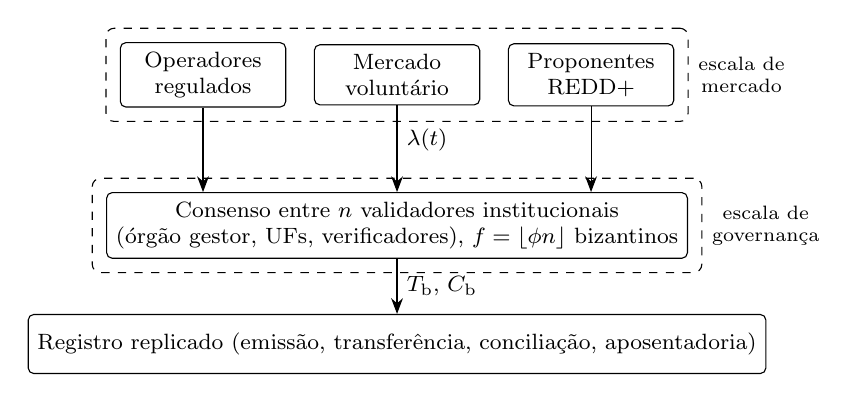
\begin{tikzpicture}[
  font=\footnotesize,
  box/.style={draw, rounded corners=2pt, align=center, minimum width=2.1cm, minimum height=0.75cm},
  layer/.style={draw, dashed, rounded corners=3pt, inner sep=5pt},
  >={Stealth[length=2mm]}]
  \node[box] (op) {Operadores\\regulados};
  \node[box, right=0.35cm of op] (vol) {Mercado\\voluntário};
  \node[box, right=0.35cm of vol] (prop) {Proponentes\\REDD+};
  \node[box, below=1.1cm of vol, minimum width=6.8cm] (cons) {Consenso entre $n$ validadores institucionais\\(órgão gestor, UFs, verificadores), $f = \lfloor \phi n \rfloor$ bizantinos};
  \node[box, below=0.7cm of cons, minimum width=6.8cm] (led) {Registro replicado (emissão, transferência, conciliação, aposentadoria)};
  \draw[->] (op) -- (op |- cons.north);
  \draw[->] (vol) -- node[right, pos=0.4]{$\lambda(t)$} (cons);
  \draw[->] (prop) -- (prop |- cons.north);
  \draw[->] (cons) -- node[right]{$\Tb$, $\Cb$} (led);
  \begin{scope}[on background layer]
   \node[layer, fit=(op)(vol)(prop), label={[font=\scriptsize,align=center]right:escala de\\mercado}] {};
   \node[layer, fit=(cons), label={[font=\scriptsize,align=center]right:escala de\\governança}] {};
  \end{scope}
\end{tikzpicture}}
\caption{Registro considerado: a demanda $\lambda(t)$ é determinada pela escala de mercado, enquanto o custo de cada rodada de consenso é determinado pela escala de governança $n$.}
\label{fig:system}
\end{figure}

A separação entre as duas escalas tem uma consequência direta. Seja $B$ o número de transações por bloco. O custo de comunicação do consenso é incorrido por bloco e é aproximadamente independente de $B$, ao passo que o custo de disseminação do conteúdo do bloco cresce com $B$. Assim, o tráfego total por bloco pode ser decomposto como
\begin{equation}
\Cb(n, B) \approx \underbrace{M(n)\, s_{\mathrm{v}}}_{\text{consenso}} + \underbrace{(n-1)\, B\, s_{\mathrm{tx}}}_{\text{disseminação}},
\label{eq:decomp}
\end{equation}
em que $M(n)$ é o número de mensagens de consenso por bloco, $s_{\mathrm{v}}$ é o tamanho de uma mensagem de voto e $s_{\mathrm{tx}}$ é o tamanho médio de uma transação. A expressão \eqref{eq:decomp} indica que o volume de transações afeta sobretudo o segundo termo, linear em $n$, enquanto o termo potencialmente quadrático depende apenas da governança. Ela também implica que $\Cb$ não segue uma lei de potência única em $n$: o expoente efetivo varia entre $1$ e $2$ conforme a razão entre os dois termos, o que é levado em conta na Seção~\ref{sec:method}. A expressão é tratada como hipótese a ser testada, e não como substituta da medição.

\subsection{Modelo de Demanda do Registro Nacional}

Seja $N_{\mathrm{op}}$ o número de operadores e participantes ativos, $\kappa$ o número médio de transações de registro por participante em um período de compromisso de duração $P$ (relatos, transferências, conciliações e aposentadorias), e $\eta$ a fração dessas transações que ocorre em uma janela de duração $\Delta$ que antecede o prazo de conciliação. A taxa média e a taxa de pico são dadas por
\begin{equation}
\bar{\lambda} = \frac{N_{\mathrm{op}}\,\kappa}{P}, \qquad \lambda_{\mathrm{pico}} = \frac{\eta\, N_{\mathrm{op}}\,\kappa}{\Delta},
\label{eq:demand}
\end{equation}
respectivamente, de modo que a razão pico/média é $\rho_{\mathrm{p}} = \eta P / \Delta$. Essa carga é representada por um processo de Poisson modulado por Markov de dois estados (MMPP-2) \citep{Fischer1993}, cujo estado de alta atividade tem duração média igual à janela e ocorre, em média, uma vez por período. Dessa forma, os parâmetros do MMPP-2 ficam integralmente determinados por
\begin{gather}
\frac{1}{\sigma_{2}} = \Delta, \qquad \frac{1}{\sigma_{1}} = P - \Delta, \nonumber\\
\lambda_{2} = \lambda_{\mathrm{pico}}, \qquad \lambda_{1} = \frac{(1-\eta)\,N_{\mathrm{op}}\,\kappa}{P - \Delta},
\label{eq:mmpp}
\end{gather}
em que $\lambda_{1}$ e $\lambda_{2}$ são as taxas nos estados de baixa e de alta atividade e $1/\sigma_{1}$ e $1/\sigma_{2}$ são os respectivos tempos médios de permanência. Pode-se verificar que a fração de tempo no estado de alta atividade é $\sigma_{1}/(\sigma_{1}+\sigma_{2}) = \Delta/P$ e que a taxa média do processo,
\begin{equation}
\frac{\sigma_{2}\lambda_{1} + \sigma_{1}\lambda_{2}}{\sigma_{1} + \sigma_{2}} = \bar{\lambda},
\label{eq:meanrate}
\end{equation}
coincide com a de \eqref{eq:demand}. Há concentração da carga somente se $\eta > \Delta/P$, isto é, se $\rho_{\mathrm{p}} > 1$; para $\eta = \Delta/P$, o MMPP-2 reduz-se a um processo de Poisson. Como referência, utiliza-se um processo de Poisson com a mesma taxa média $\bar{\lambda}$, o que permite isolar o efeito da concentração temporal do efeito da intensidade da carga \citep{Paxson1995}.

Uma vez que a regulamentação do SBCE ainda definirá os setores abrangidos e a duração dos períodos de compromisso \citep{Lei15042}, os valores de $N_{\mathrm{op}}$, $\kappa$, $\eta$, $\Delta$ e $P$ não são fixados em um único cenário. A taxa média é variada em três ordens de grandeza, e a razão pico/média $\rho_{\mathrm{p}}$ é avaliada em um experimento de sensibilidade (Seção~\ref{sec:method}). As fronteiras de viabilidade são, assim, apresentadas como função de $\bar{\lambda}$ para cada valor de $\rho_{\mathrm{p}}$ avaliado, e não para um cenário regulatório arbitrário. \chk{Definir as faixas de $N_{\mathrm{op}}$, $\kappa$, $\eta$, $\Delta$ e $P$ e as fontes empregadas.}

\subsection{Métricas e Critérios de Viabilidade}

As métricas consideradas são o tempo médio de finalização de bloco, $\Tb$, e o tráfego total por bloco, $\Cb$, conforme \citep{Caburlao2025reic,Caburlao2026clei}, complementadas pelo tráfego máximo por nó, $\Cn$, pela vazão sustentada, $\Th$, definida como a maior taxa de confirmação mantida sob saturação, pelo percentil 95 da latência de confirmação de transações, $\Lt$, e pela ocupação do enlace de subida mais carregado, $\Ut$, medida como a fração do tempo em que esse enlace permanece ocupado. Como o JABS modela filas de envio e de recepção por nó, $\Ut$ é obtida diretamente da simulação, e sua aproximação analítica,
\begin{equation}
\Ut \approx \frac{8\, \Cn\, \nu_{\mathrm{b}}}{\Kn},
\label{eq:util}
\end{equation}
em que $\Cn$ é expresso em bytes por bloco, $\nu_{\mathrm{b}}$ é a taxa de produção de blocos e $\Kn$ é a capacidade do enlace em bits por segundo, é utilizada apenas como verificação. Diferentemente de $\Cb$, a métrica $\Ut$ captura o nó gargalo, o que é essencial para protocolos centrados no líder, como o HotStuff.

Uma configuração é considerada viável se atender simultaneamente a três critérios, fixados antes da bateria principal:
\begin{align}
\text{(V1) estabilidade:} \quad & Q(kP) \leq \epsilon_{Q}\ \ \forall k, \nonumber\\
\text{(V2) latência:} \quad & \Lt \leq L_{\max}, \label{eq:feas}\\
\text{(V3) enlace:} \quad & \Ut \leq U_{\max}, \nonumber
\end{align}
em que $Q(kP)$ é o número de transações pendentes ao final do $k$-ésimo período de compromisso e $\epsilon_{Q}$ é uma tolerância. O critério V1 exige que o acúmulo formado durante a janela de pico seja escoado antes do período seguinte, o que é menos restritivo do que exigir $\Th \geq \lambda_{\mathrm{pico}}$, uma vez que rajadas curtas podem ser absorvidas por fila. O efeito dessa fila sobre os usuários é capturado por V2. A fronteira de viabilidade de um protocolo, $\nmax(\bar{\lambda})$, é o maior $n$ que atende a \eqref{eq:feas} para uma dada demanda, e a restrição vinculante é o primeiro critério violado quando $n$ cresce. \chk{Fixar $\epsilon_{Q}$, $L_{\max}$ (por exemplo, como fração de $\Delta$) e $U_{\max}$ (por exemplo, $0{,}7$) antes da bateria principal.}

% 05-metodologia.tex -- incluído por main-pt.tex
% =====================================================================
\section{Metodologia}
\label{sec:method}
% =====================================================================

\subsection{Projeto Experimental}

Os experimentos seguem a metodologia de \citet{Jain1991} e estão organizados em um experimento piloto, na fixação do protocolo de análise e na bateria principal. O piloto é utilizado para validar o simulador, estimar a variabilidade das respostas e determinar o número de replicações. As métricas, os níveis, os testes, o nível de significância, os limiares de \eqref{eq:feas} e a regra de recomendação são registrados antes da bateria principal.

Por transparência, registra-se que o desenho aqui descrito resulta de uma revisão do desenho inicial do estudo, motivada pela identificação da estimativa de tráfego discutida a seguir e por questionamentos sobre a escalabilidade do pBFT em escala nacional. A revisão ocorreu antes da bateria principal, e as execuções realizadas com o desenho inicial são utilizadas apenas no piloto. \chk{Declarar se algum resultado dessas execuções foi examinado antes da revisão e de que forma.}

A bateria principal compreende dois experimentos. O experimento E1 é um projeto fatorial completo com os fatores da Tabela~\ref{tab:factors}, que incluem a fração de validadores bizantinos, de modo que as fronteiras de viabilidade sejam obtidas também sob falhas. O nível $\phi = 0{,}30$ fica abaixo do limiar de um terço de todos os protocolos retidos; para $n = 4$, corresponde a $f = 1$. O experimento E2 avalia a sensibilidade à concentração da demanda, com $\rho_{\mathrm{p}}$ em três níveis, para os protocolos BFT nas combinações de $n$ e $\bar{\lambda}$ mais próximas das fronteiras obtidas em E1. Adicionalmente, os níveis $n \in \{400, 800\}$ não são utilizados em nenhum ajuste e servem exclusivamente para validar os metamodelos, em um subconjunto de células de E1 (demanda intermediária, enlace institucional); o nível $n = 400$ coincide com a maior escala mencionada na avaliação preliminar da Arq-REDD+ \chk{confirmar}. A viabilidade computacional das execuções com $n = 800$, em que o pBFT troca da ordem de $10^{6}$ mensagens por bloco, é verificada no piloto.

\begin{table}[!ht]
\caption{Fatores e níveis do experimento E1 e sua justificativa.}
\label{tab:factors}
\centering
\footnotesize
\setlength{\tabcolsep}{3pt}
\begin{tabular}{@{}lp{2.5cm}p{3.0cm}@{}}
\hline\hline
Fator & Níveis & Justificativa \\
\hline
A: Protocolo & pBFT, Tendermint, HotStuff, PoSA, PoS & Tabela~\ref{tab:req} \\
N: Validadores $n$ & 4, 16, 64, 256 & faixa de governança, razão 4 \\
D: Demanda $\bar{\lambda}$ & $\lambda_{0}$, $10\lambda_{0}$, $100\lambda_{0}$ & cenários regulatórios \eqref{eq:demand} \\
R: Regime & Poisson, MMPP-2 & concentração nos prazos \\
K: Enlace $\Kn$ & institucional, restrito & conectividade de nós remotos \\
$\Phi$: Bizantinos $\phi$ & 0; 0,30 & requisito R3 \\
\hline
\multicolumn{2}{@{}l}{Configurações} & $5\times4\times3\times2\times2\times2 = 480$ \\
\hline\hline
\end{tabular}
\end{table}

Todas as simulações são realizadas no simulador JABS \citep{Yajam2023}. A versão atual do simulador inclui o pBFT, o PoSA (Parlia) e o Casper FFG, com chegadas de transações de Poisson; a execução de E1 requer a implementação do Tendermint, do HotStuff, do gerador MMPP-2 de \eqref{eq:mmpp} e das trocas de visão do pBFT, sem as quais um líder bizantino interrompe a progressão do protocolo. \chk{Condicionado a essas implementações e à sua validação no piloto.} Os validadores bizantinos adotam o comportamento de silêncio, isto é, deixam de enviar votos e, quando líderes, deixam de propor blocos \chk{confirmar os tipos de ataque disponíveis no \texttt{ByzantineConfig}}.

Um aspecto metodológico é determinante para a validade das conclusões: o tráfego $\Cb$ é medido em nível de pacote, somando-se o tamanho de todas as mensagens efetivamente trocadas para finalizar cada bloco, para todos os protocolos. Na versão atual do simulador, o tráfego do pBFT é estimado como $2n \times 1.024$ bytes por bloco, acrescido de ruído, o que corresponde a um único nó enviando duas mensagens de 1~KiB a cada um dos demais. No JABS, porém, um voto do pBFT tem $42$ bytes ($32$ bytes de \textit{hash} e $10$ de sobrecarga). Considerando apenas os votos, o tráfego total esperado é da ordem de $2n^{2} \times 42$ bytes, de modo que a estimativa superestima o tráfego para $n \lesssim 24$ e o subestima para valores maiores, com razão da ordem de $16$ em $n = 400$. \chk{Condicionado à aceitação e à implementação da ADR-0001.} Cada configuração é executada com $r$ replicações independentes, com sementes distintas e descarte do transiente inicial \citep{Law2015}, em que $r$ é obtido a partir do piloto de modo que a semiamplitude do intervalo de confiança de $95\%$ das respostas estocásticas não exceda $5\%$ da média \citep{Jain1991}:
\begin{equation}
r = \max_{m}\left\lceil \left( \frac{z_{0,975}\, s_{m}}{0{,}05\, \bar{y}_{m}} \right)^{2} \right\rceil.
\label{eq:reps}
\end{equation}

Antes da bateria principal, o simulador é validado em duas etapas. Na primeira, reproduzem-se os cenários de \citep{Caburlao2026clei} para o PoSA e o PoS. Na segunda, verifica-se que o número de mensagens de consenso medido para o pBFT com $n \in \{4, 16, 64\}$ coincide com o valor esperado pela especificação do protocolo, o que confirma a correção da instrumentação.

\subsection{Elasticidades e Validação Fora da Faixa}

A questão central do trabalho, isto é, se a viabilidade é mais sensível à escala de governança ou à de mercado, é respondida por elasticidades, que são adimensionais e não dependem da amplitude dos níveis escolhidos. Para o tráfego total, ajusta-se, para cada protocolo e cada combinação dos fatores R, K e $\Phi$, o metamodelo de dois termos sugerido por \eqref{eq:decomp},
\begin{equation}
\Cb = \alpha\, n^{\,b} + \beta\, (n-1)\, \bar{B},
\label{eq:cbmodel}
\end{equation}
por mínimos quadrados não lineares, em que $\bar{B}$ é o número médio de transações por bloco medido e $b$ é o expoente do termo de consenso, esperado próximo de $2$ para pBFT e Tendermint e de $1$ para HotStuff no caso normal \eqref{eq:mpbft}. Para $\Tb$, $\Lt$ e $\Ut$, ajusta-se o metamodelo
\begin{multline}
\ln y = a + b \ln n + c \ln \bar{\lambda} + d \ln n \ln \bar{\lambda} \\
+ \textstyle\sum_{X \in \{R, K, \Phi\}} g_{X}\, \mathbb{1}_{X} + e,
\label{eq:scaling}
\end{multline}
em que $\mathbb{1}_{X}$ são variáveis indicadoras dos níveis de R, K e $\Phi$. As elasticidades em relação às duas escalas são então
\begin{equation}
\varepsilon_{n} = \frac{\partial \ln y}{\partial \ln n}, \qquad \varepsilon_{\lambda} = \frac{\partial \ln y}{\partial \ln \bar{\lambda}},
\label{eq:elast}
\end{equation}
avaliadas no centro da faixa de governança e de demanda, com intervalos de confiança obtidos por \textit{bootstrap} sobre as replicações. Os metamodelos são utilizados para predizer as respostas em $n \in \{400, 800\}$ e considerados válidos para extrapolação se os valores simulados nesses níveis estiverem contidos nos intervalos de predição de $95\%$ e o erro percentual absoluto médio for inferior a $10\%$ \citep{Kleijnen2015}. \chk{Limiar a fixar antes da bateria principal.} Para o PoS e o PoSA, $n$ representa o número de validadores que participam da produção e da finalização dos blocos, e não são formuladas expectativas teóricas para os expoentes.

\subsection{Testes de Efeitos por Análise de Variância}

A ANOVA é utilizada para testar a existência dos efeitos e, sobretudo, das interações que determinam se a ordenação dos protocolos muda com as condições de operação. Como os fatores são escolhidos deliberadamente, adota-se um modelo de efeitos fixos. Para cada resposta estocástica $m \in \{\Tb, \Lt, \Ut\}$, a observação $y$ da $l$-ésima replicação na célula $c$ do projeto é modelada como
\begin{equation}
y^{(\theta)}_{cl} = \mu + \sum_{E \in \mathcal{E}} \tau_{E}(c) + \varepsilon_{cl},
\label{eq:anova}
\end{equation}
em que $\mathcal{E}$ é o conjunto dos efeitos principais e das interações entre os fatores da Tabela~\ref{tab:factors}, $\tau_{E}(c)$ é o efeito $E$ na célula $c$, sujeito a restrições de soma zero, e $y^{(\theta)}$ é a transformação de Box--Cox \citep{BoxCox1964},
\begin{equation}
y^{(\theta)} = \begin{cases} (y^{\theta}-1)/\theta, & \theta \neq 0, \\ \ln y, & \theta = 0, \end{cases}
\label{eq:boxcox}
\end{equation}
necessária porque as respostas são positivas, assimétricas e variam em várias ordens de grandeza entre protocolos, o que torna os efeitos multiplicativos \citep{Jain1991,Montgomery2017}. O tráfego $\Cb$ não é submetido à ANOVA, pois, para os protocolos BFT, a contagem de mensagens por bloco é praticamente determinística e a variância entre replicações tende a zero, o que tornaria os testes degenerados; para essa resposta, a análise baseia-se exclusivamente em \eqref{eq:cbmodel}.

A análise segue cinco etapas: (i) testes $F$ para todos os efeitos, com somas de quadrados coincidentes por se tratar de projeto balanceado; (ii) verificação da normalidade dos resíduos por gráficos quantil--quantil, complementados pelo teste de Shapiro--Wilk \citep{Shapiro1965} apenas nas células com até $5.000$ observações, e da homogeneidade das variâncias pelo teste de Brown--Forsythe \citep{Brown1974}; (iii) repetição da inferência com erros-padrão robustos à heterocedasticidade (HC3) \citep{Long2000} e por uma análise fatorial não paramétrica com transformação de postos alinhados (ART) \citep{Wobbrock2011}, que preserva os testes de interação, sendo um efeito considerado estabelecido apenas se significativo nas três análises; (iv) comparações entre protocolos dentro de cada nível dos fatores com que interagem, pelo procedimento de Games--Howell \citep{Games1976}, com controle da taxa de erro por família pelo procedimento de Holm \citep{Holm1979} a $\alpha = 0{,}05$; e (v) tamanhos de efeito pela estatística
\begin{equation}
\omega^{2}_{E} = \frac{SS_{E} - \mathit{gl}_{E}\, MS_{\mathrm{err}}}{SST + MS_{\mathrm{err}}}
\label{eq:omega}
\end{equation}
\citep{Olejnik2003}. As parcelas de variação $SS_{E}/SST$ \citep{Jain1991} são reportadas de forma descritiva e não são utilizadas para comparar a importância de fatores cujas faixas de níveis foram fixadas arbitrariamente, papel que cabe às elasticidades \eqref{eq:elast}. Nenhum fator é descartado com base apenas em um efeito principal fraco quando suas interações são significativas.

\subsection{Fronteiras de Viabilidade e Recomendação}

As fronteiras $\nmax(\bar{\lambda})$ são obtidas, para cada protocolo e cada combinação de $\rho_{\mathrm{p}}$, K e $\Phi$, pela inversão dos metamodelos validados em relação aos critérios \eqref{eq:feas}, e confirmadas por simulação direta em pontos imediatamente abaixo e acima da fronteira estimada. A recomendação de protocolo para um cenário de governança $n$ e de demanda $\bar{\lambda}$ segue três etapas, fixadas antes da bateria principal: (i) admissibilidade, que exige o atendimento integral de R1--R4 e um limiar de tolerância superior a $\phi$; (ii) viabilidade pelos critérios \eqref{eq:feas}; e (iii) entre os protocolos admissíveis e viáveis, preferência pelo menor $\Lt$, por ser a métrica percebida pelos participantes do mercado, com desempate, quando os intervalos de confiança se sobrepõem, pela maior margem $\nmax(\bar{\lambda})/n$, que favorece configurações capazes de acomodar a expansão da governança sem reengenharia do registro.

% 06-resultados.tex -- incluído por main-pt.tex
% =====================================================================
\section{Resultados Numéricos e Discussões}
\label{sec:results}
% =====================================================================

Nesta seção, os resultados numéricos da bateria principal são apresentados juntamente com a análise estatística correspondente. Todos os resultados são reportados como médias com intervalos de confiança de $95\%$ sobre $r = $ \tbd{valor} replicações, e assume-se, salvo indicação em contrário, $\lambda_{0} = $ \tbd{valor} transações por segundo e $\rho_{\mathrm{p}} = $ \tbd{valor}.

\subsection{Validação do Simulador e Efeito da Medição do Tráfego}

\begin{figure}[!ht]
\centering
\figplaceholder{4.5cm}{Fig. 2 -- $\Cb$ do pBFT versus $n$ (escala log-log): estimativa em forma fechada versus medição em nível de pacote, $n$ de 4 a 400, com o ponto de cruzamento indicado.}
\caption{Tráfego de finalização de bloco do pBFT versus número de validadores: estimativa em forma fechada da versão atual do simulador e medição em nível de pacote.}
\label{fig:artifact}
\end{figure}

\tbd{Resultado da reprodução dos cenários de \citep{Caburlao2026clei} para PoSA e PoS e da verificação da contagem de mensagens do pBFT.} A Figura~\ref{fig:artifact} compara, para o pBFT, a estimativa em forma fechada com o tráfego medido em nível de pacote. Pode-se observar que \tbd{descrever: a estimativa cresce com expoente 1, enquanto a medição cresce com expoente $\hat{b} = $ ...; localizar o cruzamento, esperado próximo de $n = 24$}. Isso é esperado, uma vez que a estimativa supõe mensagens de 1~KiB enviadas por um único nó, enquanto a medição soma votos de $42$ bytes trocados em duas fases de todos para todos \eqref{eq:mpbft}. Portanto, a estimativa não apenas erra o valor absoluto, como também a forma do crescimento, que é o que determina a viabilidade em escala.

\subsection{Leis de Escala e Elasticidades}

\begin{figure}[!ht]
\centering
\figplaceholder{4.5cm}{Fig. 3 -- $\Cb$ e $\Cn$ versus $n$ (log-log) para os cinco protocolos, com ajustes de \eqref{eq:cbmodel} e pontos de validação em 400 e 800.}
\caption{Tráfego total por bloco e tráfego máximo por nó versus número de validadores, com os metamodelos ajustados e os pontos de validação fora da faixa de ajuste.}
\label{fig:scaling}
\end{figure}

A Figura~\ref{fig:scaling} apresenta o tráfego total e o tráfego do nó mais carregado em função de $n$. Pode-se observar que \tbd{expoentes $\hat{b}$ do termo de consenso por protocolo e comparação com a teoria}. Em particular, \tbd{HotStuff: expoente do tráfego total próximo de 1, mas tráfego do líder também linear em $n$; discutir se o líder se torna o gargalo}. Os pontos de validação em $n \in \{400, 800\}$ \tbd{estão/não estão contidos nos intervalos de predição; MAPE}.

\begin{table}[!ht]
\caption{Elasticidades em relação à governança ($\varepsilon_{n}$) e à demanda ($\varepsilon_{\lambda}$), avaliadas no centro das faixas, com $\phi = 0$ e enlace institucional (\textcolor{red}{?}: pendente).}
\label{tab:elast}
\centering
\footnotesize
\setlength{\tabcolsep}{3pt}
\begin{tabular}{@{}lcccccc@{}}
\hline\hline
\multirow{2}{*}{Protocolo} & \multicolumn{2}{c}{$\Cb$} & \multicolumn{2}{c}{$\Lt$} & \multicolumn{2}{c}{$\Ut$} \\
 & $\varepsilon_{n}$ & $\varepsilon_{\lambda}$ & $\varepsilon_{n}$ & $\varepsilon_{\lambda}$ & $\varepsilon_{n}$ & $\varepsilon_{\lambda}$ \\
\hline
pBFT       & \tbdc & \tbdc & \tbdc & \tbdc & \tbdc & \tbdc \\
Tendermint & \tbdc & \tbdc & \tbdc & \tbdc & \tbdc & \tbdc \\
HotStuff   & \tbdc & \tbdc & \tbdc & \tbdc & \tbdc & \tbdc \\
PoSA       & \tbdc & \tbdc & \tbdc & \tbdc & \tbdc & \tbdc \\
PoS        & \tbdc & \tbdc & \tbdc & \tbdc & \tbdc & \tbdc \\
\hline\hline
\end{tabular}
\end{table}

A Tabela~\ref{tab:elast} apresenta as elasticidades. \tbd{Comparar $\varepsilon_{n}$ e $\varepsilon_{\lambda}$ por protocolo e resposta: esta é a evidência central para a hipótese de trabalho.}

\subsection{Restrição Vinculante e Fronteiras de Viabilidade}

\begin{figure}[!ht]
\centering
\figplaceholder{5cm}{Fig. 4 -- $\nmax$ versus $\bar{\lambda}$ (log-log) para cada protocolo, enlace e $\phi$; faixa de governança ($n \le 256$) sombreada; marcador indicando a restrição vinculante (V1, V2 ou V3).}
\caption{Fronteiras de viabilidade $\nmax(\bar{\lambda})$ para cada protocolo, capacidade de enlace e fração bizantina, com a faixa de governança destacada e a restrição vinculante indicada.}
\label{fig:frontier}
\end{figure}

A Figura~\ref{fig:frontier} ilustra as fronteiras de viabilidade. \tbd{Para cada protocolo: em que demanda a fronteira cruza a faixa de governança; qual critério se esgota primeiro; deslocamento da fronteira com $\phi = 0{,}30$ e com enlace restrito.} \tbd{Relação entre a fronteira e o dimensionamento territorial ($n \approx 10^5$).}

\subsection{Efeito da Concentração da Demanda}

\tbd{Experimento E2: deslocamento de $\Lt$ e de $\nmax$ com $\rho_{\mathrm{p}}$; comparar com o Poisson de mesma $\bar{\lambda}$ e discutir se uma avaliação com Poisson superestimaria a fronteira.}

\subsection{Testes de Efeitos e Interações}

\begin{table*}[!ht]
\caption{Efeitos e interações das respostas estocásticas de E1: valores-$p$ das análises clássica e ART e tamanho de efeito $\omega^{2}_{E}$. Apenas efeitos significativos nas três análises (clássica, HC3 e ART) são apresentados.}
\label{tab:anova}
\centering
\small
\begin{tabular}{@{}lccccccccc@{}}
\hline\hline
\multirow{2}{*}{Efeito} & \multicolumn{3}{c}{$\Tb$} & \multicolumn{3}{c}{$\Lt$} & \multicolumn{3}{c}{$\Ut$} \\
 & $p_{F}$ & $p_{\mathrm{ART}}$ & $\omega^{2}_{E}$ & $p_{F}$ & $p_{\mathrm{ART}}$ & $\omega^{2}_{E}$ & $p_{F}$ & $p_{\mathrm{ART}}$ & $\omega^{2}_{E}$ \\
\hline
A$\times$N        & \tbdc & \tbdc & \tbdc & \tbdc & \tbdc & \tbdc & \tbdc & \tbdc & \tbdc \\
A$\times$R        & \tbdc & \tbdc & \tbdc & \tbdc & \tbdc & \tbdc & \tbdc & \tbdc & \tbdc \\
A$\times\Phi$     & \tbdc & \tbdc & \tbdc & \tbdc & \tbdc & \tbdc & \tbdc & \tbdc & \tbdc \\
A$\times$K        & \tbdc & \tbdc & \tbdc & \tbdc & \tbdc & \tbdc & \tbdc & \tbdc & \tbdc \\
D$\times$R        & \tbdc & \tbdc & \tbdc & \tbdc & \tbdc & \tbdc & \tbdc & \tbdc & \tbdc \\
\hline\hline
\end{tabular}
\end{table*}

A Tabela~\ref{tab:anova} apresenta os efeitos e as interações estabelecidos. \tbd{$\hat\theta$ de Box--Cox; verificações de premissas; concordância entre as três análises (incluir $p_{\mathrm{HC3}}$ no texto ou em material suplementar).} \tbd{Discutir em que condições a ordenação dos protocolos se inverte (interações com A).}

\subsection{Discussão: Viabilidade em Escala Nacional}

\tbd{Responder diretamente, com base nas fronteiras, se o consenso bizantino é viável em escala nacional: (a) com governança institucional ($n \le 256$), quais protocolos são viáveis para cada faixa de demanda, com e sem validadores bizantinos; (b) com dimensionamento territorial, se algum protocolo bizantino plano é viável ou se a alternativa é uma arquitetura hierárquica \citep{Amir2010}; (c) implicações para a regulamentação do registro central do SBCE.}

\subsection{Limitações}

\tbd{Avaliação por simulação; demanda paramétrica até a regulamentação do SBCE; um único comportamento bizantino (silêncio); avaliação de segurança restrita ao limiar de tolerância; arquiteturas hierárquicas discutidas, mas não simuladas; riscos de contratos inteligentes e oráculos fora do escopo \citep{GhiyamiPour2025,Rahman2023}.}

% 07-conclusoes.tex -- incluído por main-pt.tex
% =====================================================================
\section{Conclusões}
\label{sec:conclusion}
% =====================================================================

Esta contribuição investigou a viabilidade do consenso bizantino em um registro nacional de créditos de carbono baseado em blockchain. A questão foi formulada em termos de duas escalas distintas: a escala de governança, que determina o número de validadores e o custo de comunicação de cada rodada de consenso, e a escala de mercado, que determina a demanda de transações e sua concentração em torno dos prazos de conciliação. Os protocolos avaliados foram selecionados a partir de requisitos do domínio, o tráfego de consenso foi medido em nível de pacote, validadores bizantinos foram incluídos no projeto fatorial, e as elasticidades em relação às duas escalas foram estimadas por metamodelos validados fora da faixa de ajuste, com as interações testadas por ANOVA. Mostrou-se que \tbd{principal achado sobre as elasticidades e a restrição vinculante} e que \tbd{fronteiras de viabilidade na faixa de governança, com e sem falhas}, o que \tbd{confirma/refuta} a hipótese de que a viabilidade de um registro nacional depende mais do desenho de governança do que do volume de transações. Em qualquer caso, as fronteiras obtidas podem subsidiar a regulamentação do registro central do SBCE, ao explicitar quantos validadores um registro pode comportar para cada nível de demanda. Possíveis extensões deste trabalho envolvem a simulação de arquiteturas hierárquicas de consenso, a inclusão de outros comportamentos bizantinos e a calibração do modelo de demanda com os dados dos primeiros períodos de compromisso do SBCE. Outra direção de pesquisa poderia investigar o impacto dos oráculos de MRV sobre a demanda e a segurança do registro.


% 08-declaracoes.tex -- incluído por main-pt.tex
% =====================================================================
\begin{declarations}

\begin{acknowledgements}
\chk{Opcional.}
\end{acknowledgements}

\begin{contributions}
\chk{Declaração CRediT a ser definida pelos autores; sugestão a confirmar: FRF contribuiu para a concepção do estudo, o projeto experimental e a análise estatística. MCC desenvolveu a arquitetura Arq-REDD+ e os cenários de simulação. CKSR supervisionou o trabalho. Todos os autores leram e aprovaram o manuscrito final.}
\end{contributions}

\begin{interests}
Os autores declaram não haver conflitos de interesse.
\end{interests}

\begin{materials}
O simulador e os scripts utilizados no presente estudo estão disponíveis em \url{https://github.com/frfreire/Arq-REDD-Framework}. \chk{Adicionar o link dos dados e do protocolo de análise registrado (por exemplo, DOI no OSF ou Zenodo).}
\end{materials}

\begin{funding}
\chk{Opcional.}
\end{funding}

\begin{furtherinformation}
Esta pesquisa não envolveu participantes humanos e, portanto, não exigiu aprovação por comitê de ética. \chk{Declarar o uso de ferramentas de IA generativa, se aplicável.}
\end{furtherinformation}

\end{declarations}



\bibliographystyle{apalike-sol}
\bibliography{refs}

\end{document}
